\documentclass[20pt,a4paper]{article}
\usepackage{amsmath}
\usepackage{amsfonts}
\usepackage{amssymb}
\usepackage{graphicx}
\usepackage[left=2cm,right=2cm,top=2cm,bottom=2cm]{geometry}

\author{Aritra Das}
\title{The Quadratic Reciprocity Law}

\date{June 17, 2022}

\begin{document}

\maketitle

\section{Basics}
Roughly speaking The Quadratic Reciprocity Law deals with the solvability of quadratic congruences.Therefore it seems reasonable to begin with considering the congruence:
\begin{equation}
    ax^2 + bx + c \equiv 0 \pmod{p} \ where \ p\ is \ an \ odd \ prime
\end{equation}
\section{A Simpler Form}
The equations can be further simplified as follows \\
\[
\quad 4a(ax^2 + bx + c) \equiv 0 \pmod{p}  = 1
\]
as $\gcd(4a,p) = 1$,
or \\
\[
\quad 4a(ax^2 + bx + c) = (2ax+b)^2 - (b^2 - 4ac) \\
\]
Let $y = 2ax + b$ and $d = b^2 - 4ac$ to get
\begin{equation}
    y^2 \equiv d \pmod{p}
\end{equation}
\section{What is Quadratic Residue}
Let p be an odd prime and $gcd(a,p)=1$. If the Quadratic congruence $x^2 \equiv a \pmod{p}$ has a solution then a is said to be a \textbf{quadratic residue of p}. Otherwise,  a is called a \textbf{quadratic nonresidue of p}.
\section{Euler's Criterion}
    Let p be an odd prime and $\gcd(a,p)=1$. Then a is a quadratic residue of p if and only if 
\begin{equation}
   a^{(p-1)/2} \equiv 1 \pmod{p} 
\end{equation}
Proof is based on Fermat's theorem
\section{Legendre Symbol}    
\subsection{Definition of the symbol}
Let p be an odd prime and let $\gcd(a,p)=1$. The \textbf{Legendre symbol} $(a/p)$ is defined by
\[
(a/p) =
\left\{
\begin{array}{ll}
    \ \ 1 & \text{if a is a quadratic residue of p }  \\
   -1 & \text{if a is a quadratic non-residue of p} \\
\end{array}
\right.
\]


Few important properties of Legendre Symbol

\begin{itemize}
\item If $a \equiv b \pmod{p}$, then $\left(\frac{a}{p}\right) = \left(\frac{b}{p}\right)$.
\item $(a^2/p)=1$
\item $(a/p) \equiv a^{(p-1)/2} \pmod{p}$
\item $(ab/p) = (a/p)(b/p)$
\item $(1/p)=1 and (-1/p) = (-1)^{(p-1)/2}.$
\end{itemize}
\section{Gauss Lemma}
The idea of proof is taken from~\cite{enwiki:1152801587}.
Let p be an odd prime and let $\gcd(a,p) =1$. If n denotes the number of integers in the set
\[
S = \{a, 2a, 3a, \dots, \frac{p-1}{2}a\}
\]
whose remainder upon division by p exceed p/2, then
\begin{equation}
   (a/p)=(-1)^{n} \label{eqn:gauss}
\end{equation}
\section{Quadratic Reciprocity Law}
Let p and q be distinct odd primes, so that both of the Legendre symbols(p/q) and (p/q) are defined.\\
Quite natural to think if we can relate (p/q) and (q/p) somehow\\
This is what the \textbf{Quadratic reciprocity Law} tells us
\begin{equation}
    (p/q)(q/p)=(-1)^{\frac{p-1}{2}\frac{q-1}{2}}
\end{equation}
\subsection{Proof}
This proof is taken from~\cite{enwiki:1140127449}.
Consider a rectangular box in the $xy$ coordinate plane whose vertices are (0,0),(0,q/2),(p/2,0),(p/2,q/2) Let R denote the  region within this rectangle, not including any of the bounding lines.The General plan of attack is to count the number of lattice points (that is, the points whose coordinates are integers) inside R in two different ways.
Because p and q are both odd, the lattice points in R consist of all points (n,m), where $l \leq n \leq \frac{p-1}{2}$ and $l \leq m \leq \frac{q-1}{2}$; clearly , the number of such points is 
\[
        \frac{p-1}{2}.\frac{q-1}{2}
\]
Now the diagonal D from $(0,0)$ to $(p/2,q/2)$ has an equation $y=(q/p)x$ ,or equivalently $py=qx$. \\
Refer to figure\ref{fig:image}\\
Because $\gcd(p,q)=1$, none of the lattice points inside R will lie on D.For p must divide the x coordinate of any lattice point on the line $py=qx$, and q must divide its y coordinate; there are no such points in R.Suppose T1 denotes tthe portion of R below the diagonal D, and T2 denotes the portion above. By what we have just seen, it suffices to count the lattice points inside each of these triangles.
The number of points in the interval 0 < y <$kq/p$ is equal to $[kq/p]$. Thus, for $1\leq k \leq (p-1)/2$, there are precisely $[kq/p]$ lattice points above the point $(k,0)$ and below D; in other words, lying on the vertical line segment from $(k,0)$ to $(k,kq/p)$. It follows that the total number of lattice points contained in $T_1$ is
\[
\sum_{k=1}^{(p-1)/2} [\frac{kq}{p}]
\]

A similar calculations, with the roles of p and q interchanged, shows that the number of lattice points within $T_2$ is 
\[
\sum_{j=1}^{(q-1)/2} [\frac{jp}{q}]
\]
This accounts for all of the lattice points inside R, so that
\[
\frac{p-1}{2}.\frac{q-1}{2} = \sum_{j=1}^{(q-1)/2} [\frac{jp}{q}] + \sum_{k=1}^{(p-1)/2} [\frac{kq}{p}]
\]
Now Finally Equation  \ref{eqn:gauss} to finish the proof 
\[
(p/q)(q/p)=(-1)^{\sum_{k=1}^{(p-1)/2} [\frac{kq}{p}]} .(-1)^{\sum_{j=1}^{(q-1)/2} [\frac{jp}{q}]} \\
\]
\[
\quad =(-1)^{\sum_{k=1}^{(p-1)/2} [\frac{kq}{p}] + \sum_{j=1}^{(q-1)/2} [\frac{jp}{q}]}
\]
\[
=(-1)^{[\frac{p-1}{2}] . \frac{q-1}{2}}
\]
\textbf{THIS CONCLUDES THE PROOF OF THE QUADRATIC RECIPROCITY LAW}
\begin{figure}
    \centering
    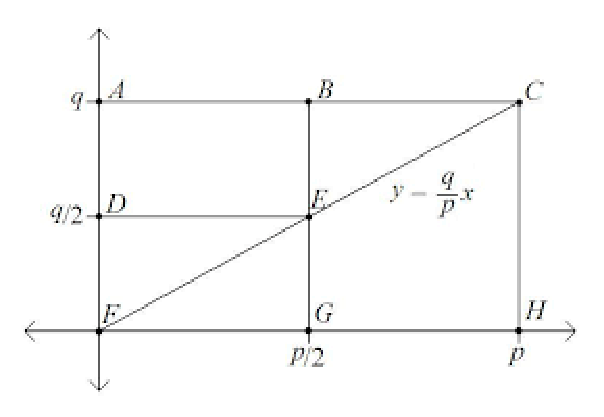
\includegraphics[scale=0.7]{quadimg2.eps}
    \caption{The rectangular box with the diagonal py=qx}
    \label{fig:image}
\end{figure}
\section{Conclusion}
The \textbf{Quadratic Reciprocity Law} is very powerful in solving many types of quadratic congruences
\bibliography{ref.bib}
\bibliographystyle{plain}
\end{document}
